
%% bare_jrnl.tex
%% V1.4b
%% 2015/08/26
%% by Michael Shell
%% see http://www.michaelshell.org/
%% for current contact information.
%%
%% This is a skeleton file demonstrating the use of IEEEtran.cls
%% (requires IEEEtran.cls version 1.8b or later) with an IEEE
%% journal paper.
%%
%% Support sites:
%% http://www.michaelshell.org/tex/ieeetran/
%% http://www.ctan.org/pkg/ieeetran
%% and
%% http://www.ieee.org/ 

%%*************************************************************************
%% Legal Notice:
%% This code is offered as-is without any warranty either expressed or
%% implied; without even the implied warranty of MERCHANTABILITY or
%% FITNESS FOR A PARTICULAR PURPOSE! 
%% User assumes all risk.
%% In no event shall the IEEE or any contributor to this code be liable for
%% any damages or losses, including, but not limited to, incidental,
%% consequential, or any other damages, resulting from the use or misuse
%% of any information contained here.
%%
%% All comments are the opinions of their respective authors and are not
%% necessarily endorsed by the IEEE.
%%
%% This work is distributed under the LaTeX Project Public License (LPPL)
%% ( http://www.latex-project.org/ ) version 1.3, and may be freely used,
%% distributed and modified. A copy of the LPPL, version 1.3, is included
%% in the base LaTeX documentation of all distributions of LaTeX released
%% 2003/12/01 or later.
%% Retain all contribution notices and credits.
%% ** Modified files should be clearly indicated as such, including  **
%% ** renaming them and changing author support contact information. **
%%*************************************************************************


% *** Authors should verify (and, if needed, correct) their LaTeX system  ***
% *** with the testflow diagnostic prior to trusting their LaTeX platform ***
% *** with production work. The IEEE's font choices and paper sizes can   ***
% *** trigger bugs that do not appear when using other class files.       ***                          ***
% The testflow support page is at:
% http://www.michaelshell.org/tex/testflow/



\documentclass[journal]{IEEEtran}
%
% If IEEEtran.cls has not been installed into the LaTeX system files,
% manually specify the path to it like:
% \documentclass[journal]{../sty/IEEEtran}





% Some very useful LaTeX packages include:
% (uncomment the ones you want to load)


% *** MISC UTILITY PACKAGES ***
%
%\usepackage{ifpdf}
% Heiko Oberdiek's ifpdf.sty is very useful if you need conditional
% compilation based on whether the output is pdf or dvi.
% usage:
% \ifpdf
%   % pdf code
% \else
%   % dvi code
% \fi
% The latest version of ifpdf.sty can be obtained from:
% http://www.ctan.org/pkg/ifpdf
% Also, note that IEEEtran.cls V1.7 and later provides a builtin
% \ifCLASSINFOpdf conditional that works the same way.
% When switching from latex to pdflatex and vice-versa, the compiler may
% have to be run twice to clear warning/error messages.






% *** CITATION PACKAGES ***
%
%\usepackage{cite}
% cite.sty was written by Donald Arseneau
% V1.6 and later of IEEEtran pre-defines the format of the cite.sty package
% \cite{} output to follow that of the IEEE. Loading the cite package will
% result in citation numbers being automatically sorted and properly
% "compressed/ranged". e.g., [1], [9], [2], [7], [5], [6] without using
% cite.sty will become [1], [2], [5]--[7], [9] using cite.sty. cite.sty's
% \cite will automatically add leading space, if needed. Use cite.sty's
% noadjust option (cite.sty V3.8 and later) if you want to turn this off
% such as if a citation ever needs to be enclosed in parenthesis.
% cite.sty is already installed on most LaTeX systems. Be sure and use
% version 5.0 (2009-03-20) and later if using hyperref.sty.
% The latest version can be obtained at:
% http://www.ctan.org/pkg/cite
% The documentation is contained in the cite.sty file itself.






% *** GRAPHICS RELATED PACKAGES ***
%
\ifCLASSINFOpdf
  % \usepackage[pdftex]{graphicx}
  % declare the path(s) where your graphic files are
  % \graphicspath{{../pdf/}{../jpeg/}}
  % and their extensions so you won't have to specify these with
  % every instance of \includegraphics
  % \DeclareGraphicsExtensions{.pdf,.jpeg,.png}
\else
  % or other class option (dvipsone, dvipdf, if not using dvips). graphicx
  % will default to the driver specified in the system graphics.cfg if no
  % driver is specified.
  % \usepackage[dvips]{graphicx}
  % declare the path(s) where your graphic files are
  % \graphicspath{{../eps/}}
  % and their extensions so you won't have to specify these with
  % every instance of \includegraphics
  % \DeclareGraphicsExtensions{.eps}
\fi
% graphicx was written by David Carlisle and Sebastian Rahtz. It is
% required if you want graphics, photos, etc. graphicx.sty is already
% installed on most LaTeX systems. The latest version and documentation
% can be obtained at: 
% http://www.ctan.org/pkg/graphicx
% Another good source of documentation is "Using Imported Graphics in
% LaTeX2e" by Keith Reckdahl which can be found at:
% http://www.ctan.org/pkg/epslatex
%
% latex, and pdflatex in dvi mode, support graphics in encapsulated
% postscript (.eps) format. pdflatex in pdf mode supports graphics
% in .pdf, .jpeg, .png and .mps (metapost) formats. Users should ensure
% that all non-photo figures use a vector format (.eps, .pdf, .mps) and
% not a bitmapped formats (.jpeg, .png). The IEEE frowns on bitmapped formats
% which can result in "jaggedy"/blurry rendering of lines and letters as
% well as large increases in file sizes.
%
% You can find documentation about the pdfTeX application at:
% http://www.tug.org/applications/pdftex





% *** MATH PACKAGES ***
%
%\usepackage{amsmath}
% A popular package from the American Mathematical Society that provides
% many useful and powerful commands for dealing with mathematics.
%
% Note that the amsmath package sets \interdisplaylinepenalty to 10000
% thus preventing page breaks from occurring within multiline equations. Use:
%\interdisplaylinepenalty=2500
% after loading amsmath to restore such page breaks as IEEEtran.cls normally
% does. amsmath.sty is already installed on most LaTeX systems. The latest
% version and documentation can be obtained at:
% http://www.ctan.org/pkg/amsmath




% *** SPECIALIZED LIST PACKAGES ***
%
%\usepackage{algorithmic}
% algorithmic.sty was written by Peter Williams and Rogerio Brito.
% This package provides an algorithmic environment fo describing algorithms.
% You can use the algorithmic environment in-text or within a figure
% environment to provide for a floating algorithm. Do NOT use the algorithm
% floating environment provided by algorithm.sty (by the same authors) or
% algorithm2e.sty (by Christophe Fiorio) as the IEEE does not use dedicated
% algorithm float types and packages that provide these will not provide
% correct IEEE style captions. The latest version and documentation of
% algorithmic.sty can be obtained at:
% http://www.ctan.org/pkg/algorithms
% Also of interest may be the (relatively newer and more customizable)
% algorithmicx.sty package by Szasz Janos:
% http://www.ctan.org/pkg/algorithmicx




% *** ALIGNMENT PACKAGES ***
%
%\usepackage{array}
% Frank Mittelbach's and David Carlisle's array.sty patches and improves
% the standard LaTeX2e array and tabular environments to provide better
% appearance and additional user controls. As the default LaTeX2e table
% generation code is lacking to the point of almost being broken with
% respect to the quality of the end results, all users are strongly
% advised to use an enhanced (at the very least that provided by array.sty)
% set of table tools. array.sty is already installed on most systems. The
% latest version and documentation can be obtained at:
% http://www.ctan.org/pkg/array


% IEEEtran contains the IEEEeqnarray family of commands that can be used to
% generate multiline equations as well as matrices, tables, etc., of high
% quality.




% *** SUBFIGURE PACKAGES ***
%\ifCLASSOPTIONcompsoc
%  \usepackage[caption=false,font=normalsize,labelfont=sf,textfont=sf]{subfig}
%\else
%  \usepackage[caption=false,font=footnotesize]{subfig}
%\fi
% subfig.sty, written by Steven Douglas Cochran, is the modern replacement
% for subfigure.sty, the latter of which is no longer maintained and is
% incompatible with some LaTeX packages including fixltx2e. However,
% subfig.sty requires and automatically loads Axel Sommerfeldt's caption.sty
% which will override IEEEtran.cls' handling of captions and this will result
% in non-IEEE style figure/table captions. To prevent this problem, be sure
% and invoke subfig.sty's "caption=false" package option (available since
% subfig.sty version 1.3, 2005/06/28) as this is will preserve IEEEtran.cls
% handling of captions.
% Note that the Computer Society format requires a larger sans serif font
% than the serif footnote size font used in traditional IEEE formatting
% and thus the need to invoke different subfig.sty package options depending
% on whether compsoc mode has been enabled.
%
% The latest version and documentation of subfig.sty can be obtained at:
% http://www.ctan.org/pkg/subfig




% *** FLOAT PACKAGES ***
%
%\usepackage{fixltx2e}
% fixltx2e, the successor to the earlier fix2col.sty, was written by
% Frank Mittelbach and David Carlisle. This package corrects a few problems
% in the LaTeX2e kernel, the most notable of which is that in current
% LaTeX2e releases, the ordering of single and double column floats is not
% guaranteed to be preserved. Thus, an unpatched LaTeX2e can allow a
% single column figure to be placed prior to an earlier double column
% figure.
% Be aware that LaTeX2e kernels dated 2015 and later have fixltx2e.sty's
% corrections already built into the system in which case a warning will
% be issued if an attempt is made to load fixltx2e.sty as it is no longer
% needed.
% The latest version and documentation can be found at:
% http://www.ctan.org/pkg/fixltx2e


%\usepackage{stfloats}
% stfloats.sty was written by Sigitas Tolusis. This package gives LaTeX2e
% the ability to do double column floats at the bottom of the page as well
% as the top. (e.g., "\begin{figure*}[!b]" is not normally possible in
% LaTeX2e). It also provides a command:
%\fnbelowfloat
% to enable the placement of footnotes below bottom floats (the standard
% LaTeX2e kernel puts them above bottom floats). This is an invasive package
% which rewrites many portions of the LaTeX2e float routines. It may not work
% with other packages that modify the LaTeX2e float routines. The latest
% version and documentation can be obtained at:
% http://www.ctan.org/pkg/stfloats
% Do not use the stfloats baselinefloat ability as the IEEE does not allow
% \baselineskip to stretch. Authors submitting work to the IEEE should note
% that the IEEE rarely uses double column equations and that authors should try
% to avoid such use. Do not be tempted to use the cuted.sty or midfloat.sty
% packages (also by Sigitas Tolusis) as the IEEE does not format its papers in
% such ways.
% Do not attempt to use stfloats with fixltx2e as they are incompatible.
% Instead, use Morten Hogholm'a dblfloatfix which combines the features
% of both fixltx2e and stfloats:
%
% \usepackage{dblfloatfix}
% The latest version can be found at:
% http://www.ctan.org/pkg/dblfloatfix

\usepackage{url}
\def\UrlBreaks{\do\/\do-}
\usepackage{breakurl}
\usepackage[draft,breaklinks]{hyperref}
%\usepackage{hyperref}
\usepackage{adjustbox}
\usepackage{multirow, array}
\usepackage{booktabs}
\newcommand{\ra}[1]{\renewcommand{\arraystretch}{#1}}
\usepackage{tabularx}
\usepackage{makecell}
\usepackage{float}
\newcolumntype{L}{>{\raggedright\arraybackslash}X}
\usepackage[acronym]{glossaries}
\usepackage{flushend}


%\ifCLASSOPTIONcaptionsoff
%  \usepackage[nomarkers]{endfloat}
% \let\MYoriglatexcaption\caption
% \renewcommand{\caption}[2][\relax]{\MYoriglatexcaption[#2]{#2}}
%\fi
% endfloat.sty was written by James Darrell McCauley, Jeff Goldberg and 
% Axel Sommerfeldt. This package may be useful when used in conjunction with 
% IEEEtran.cls'  captionsoff option. Some IEEE journals/societies require that
% submissions have lists of figures/tables at the end of the paper and that
% figures/tables without any captions are placed on a page by themselves at
% the end of the document. If needed, the draftcls IEEEtran class option or
% \CLASSINPUTbaselinestretch interface can be used to increase the line
% spacing as well. Be sure and use the nomarkers option of endfloat to
% prevent endfloat from "marking" where the figures would have been placed
% in the text. The two hack lines of code above are a slight modification of
% that suggested by in the endfloat docs (section 8.4.1) to ensure that
% the full captions always appear in the list of figures/tables - even if
% the user used the short optional argument of \caption[]{}.
% IEEE papers do not typically make use of \caption[]'s optional argument,
% so this should not be an issue. A similar trick can be used to disable
% captions of packages such as subfig.sty that lack options to turn off
% the subcaptions:
% For subfig.sty:
% \let\MYorigsubfloat\subfloat
% \renewcommand{\subfloat}[2][\relax]{\MYorigsubfloat[]{#2}}
% However, the above trick will not work if both optional arguments of
% the \subfloat command are used. Furthermore, there needs to be a
% description of each subfigure *somewhere* and endfloat does not add
% subfigure captions to its list of figures. Thus, the best approach is to
% avoid the use of subfigure captions (many IEEE journals avoid them anyway)
% and instead reference/explain all the subfigures within the main caption.
% The latest version of endfloat.sty and its documentation can obtained at:
% http://www.ctan.org/pkg/endfloat
%
% The IEEEtran \ifCLASSOPTIONcaptionsoff conditional can also be used
% later in the document, say, to conditionally put the References on a 
% page by themselves.




% *** PDF, URL AND HYPERLINK PACKAGES ***
%
%\usepackage{url}
% url.sty was written by Donald Arseneau. It provides better support for
% handling and breaking URLs. url.sty is already installed on most LaTeX
% systems. The latest version and documentation can be obtained at:
% http://www.ctan.org/pkg/url
% Basically, \url{my_url_here}.




% *** Do not adjust lengths that control margins, column widths, etc. ***
% *** Do not use packages that alter fonts (such as pslatex).         ***
% There should be no need to do such things with IEEEtran.cls V1.6 and later.
% (Unless specifically asked to do so by the journal or conference you plan
% to submit to, of course. )


% correct bad hyphenation here
\hyphenation{op-tical net-works semi-conduc-tor}


\begin{document}
%
% paper title
% Titles are generally capitalized except for words such as a, an, and, as,
% at, but, by, for, in, nor, of, on, or, the, to and up, which are usually
% not capitalized unless they are the first or last word of the title.
% Linebreaks \\ can be used within to get better formatting as desired.
% Do not put math or special symbols in the title.
\title{A Review of Sensor Technologies for Perception in Automated Driving}
%
%
% author names and IEEE memberships
% note positions of commas and nonbreaking spaces ( ~ ) LaTeX will not break
% a structure at a ~ so this keeps an author's name from being broken across
% two lines.
% use \thanks{} to gain access to the first footnote area
% a separate \thanks must be used for each paragraph as LaTeX2e's \thanks
% was not built to handle multiple paragraphs
%

\author{Enrique~Mart\'i, %~\IEEEmembership{Member,~IEEE,}
        Miguel \'Angel~de Miguel, %~\IEEEmembership{Fellow,~OSA,}
		Fernando~Garc\'ia,~\IEEEmembership{Member,~IEEE,}
        and~Joshu\'e~P\'erez,%~\IEEEmembership{Life~Fellow,~IEEE}% <-this % 
        %%%stops a space
\thanks{E. Mart\'i and J. P\'erez work in Fundaci\'on Tecnalia, 
	Derio, 48160 Spain. Corresponding e-mail: enrique.marti@tecnalia.com.}% <-this % stops a space
\thanks{M. de Miguel and F. Garc\'ia are in Universidad Carlos III de Madrid, 
Legan\'es, 28911, Spain}% <-this % stops a space
\thanks{Manuscript received November 30, 2018; accepted for publication March 18, 2019.}}

% note the % following the last \IEEEmembership and also \thanks - 
% these prevent an unwanted space from occurring between the last author name
% and the end of the author line. i.e., if you had this:
% 
% \author{....lastname \thanks{...} \thanks{...} }
%                     ^------------^------------^----Do not want these spaces!
%
% a space would be appended to the last name and could cause every name on that
% line to be shifted left slightly. This is one of those "LaTeX things". For
% instance, "\textbf{A} \textbf{B}" will typeset as "A B" not "AB". To get
% "AB" then you have to do: "\textbf{A}\textbf{B}"
% \thanks is no different in this regard, so shield the last } of each \thanks
% that ends a line with a % and do not let a space in before the next \thanks.
% Spaces after \IEEEmembership other than the last one are OK (and needed) as
% you are supposed to have spaces between the names. For what it is worth,
% this is a minor point as most people would not even notice if the said evil
% space somehow managed to creep in.



% The paper headers
\markboth{Journal of \LaTeX\ Class Files,~Vol.~14, No.~8, August~2015}%
{Shell \MakeLowercase{\textit{et al.}}: Bare Demo of IEEEtran.cls for IEEE Journals}
% The only time the second header will appear is for the odd numbered pages
% after the title page when using the twoside option.
% 
% *** Note that you probably will NOT want to include the author's ***
% *** name in the headers of peer review papers.                   ***
% You can use \ifCLASSOPTIONpeerreview for conditional compilation here if
% you desire.




% If you want to put a publisher's ID mark on the page you can do it like
% this:
%\IEEEpubid{0000--0000/00\$00.00~\copyright~2015 IEEE}
% Remember, if you use this you must call \IEEEpubidadjcol in the second
% column for its text to clear the IEEEpubid mark.
\IEEEoverridecommandlockouts
\IEEEpubid{\makebox[\columnwidth]{978-1-5386-5541-2/18/\$31.00~\copyright2018 IEEE \hfill} \hspace{\columnsep}\makebox[\columnwidth]{ }}


% use for special paper notices
%\IEEEspecialpapernotice{(Invited Paper)}




% make the title area
\maketitle

\IEEEpubidadjcol

% As a general rule, do not put math, special symbols or citations
% in the abstract or keywords.
\begin{abstract}
    After more than 20 years of research, ADAS are common in modern vehicles
    available in the market. Automated Driving systems, still in
    research phase and limited in their capabilities, are starting early 
    commercial tests in public roads.
    These systems rely on the information provided by on-board sensors, 
    which allow to describe the state of the vehicle, its environment and
    other actors. Selection and arrangement of sensors represent
    a key factor in the design of the system. 
    This survey reviews existing, novel and upcoming sensor technologies, 
    applied to common perception tasks for ADAS and Automated Driving.
    They are put in context making a historical review of the most
    relevant demonstrations on Automated Driving, focused on their sensing 
    setup. 
    Finally, the article presents a snapshot of the future challenges for
    sensing technologies and perception, finishing with an overview of 
    the commercial initiatives and manufacturers alliances that will show 
    future market trends in sensors technologies for Automated Vehicles.
\end{abstract}

% Note that keywords are not normally used for peerreview papers.
\begin{IEEEkeywords}
Automated Driving, LiDAR, Radar, Artificial Vision, Perception.
\end{IEEEkeywords}






% For peer review papers, you can put extra information on the cover
% page as needed:
% \ifCLASSOPTIONpeerreview
% \begin{center} \bfseries EDICS Category: 3-BBND \end{center}
% \fi
%
% For peerreview papers, this IEEEtran command inserts a page break and
% creates the second title. It will be ignored for other modes.
\IEEEpeerreviewmaketitle




\section{Introduction}
\label{sec:01-intro}

Every year more than one million people die on road accidents and several 
million more get injured \cite{world2015global}. In addition to the social cost, it also has an
important economic impact for nations worldwide. According to 
\cite{Thomas2013} the most frequent causes for car accidents in the
European Union are human related: speeding, driving under the effects of
alcohol or drugs, reckless driving, distractions or just plain misjudgments.

Automated Driving systems aim to take the human driver out of the equation. 
This makes them a tool with the potential to reduce the number of traffic 
accidents.
Based on recent developments and demonstrations around the world, there is a 
tendency to think that Automated Driving with a high level of automation will 
be available in a few years. This raises questions about its safety. 

The architecture of Automated Vehicles is usually divided into three 
categories: perception of the environment, behavior planning and motion 
execution \cite{behere2015functional}. Automated 
vehicles obtain information about their surroundings using different
sensors, such as cameras, LiDARs and radars. Raw data is processed to extract
relevant features which are the input to the following stages (behavior
planning and motion execution), that will perform tasks such as path planning,
collision avoidance or control of the vehicle among others. 

Perception is a very challenging problem for several
reasons. First, the environment is complex and highly dynamic, with some cases
involving a large number of participants (dense traffic, populated cities). 
Second, it needs to work reliably under a wide range of external conditions, 
including lighting and weather (rain, fog, snow, dust). 
Perception errors are propagated and can be the cause of severe accidents. 
Some real examples include the 2016 Tesla AutoPilot accident \cite{NTSB2017},
where a man was killed after its car crashed a truck: 
the camera failed to detect the gray truck against a bright sky while radar
detection was discarded as background noise by perception algorithms.
Later in 2018, a Tesla model X crashed a highway divider after the lane
following system failed to detect faded lines and the concrete divider was not
recognized, killing the driver \cite{NTSB2018a}.
Also in 2018, an experimental Uber vehicle killed a woman that was
crossing the road \cite{NTSB2018} in the night, dressed in dark clothes. 
Only the LiDAR provided a solid detection, that was discarded as a false
positive by perception algorithms.

Sensor technologies have been surveyed previously in the literature, 
but usually centered on ADAS implementation \cite{Yenkanchi2016,Ziebinski2016a} 
or at a general level within Automated Driving \cite{Pendleton2017}. 
One of the main contributions of this work is its focus on the relation between 
sensors and perception, which provide an integral view of the process that 
leads from raw sensor data to meaningful information for the driving task.

The content of the article is organized as follows. Section 
\ref{sec:02-sensors} reviews the sensor technologies commonly used for 
perception, its drawbacks and advantages, and related emerging 
technologies that can be used in the future. 
Section \ref{sec:03-problemsapplications} starts describing the most important 
competences in perception, to proceed with a state of the art of perception 
algorithms and techniques grouped by competences. Sensors used on each work
are enumerated, and their advantages and disadvantages are discussed. 
Section \ref{sec:04-relevantdemos} gives a perspective of the evolution of
perception in Automated Driving, presenting the most relevant works and demos
in the history of the discipline with a focus in sensor technologies used for
each one. 
Finally, section \ref{sec:06-discussion} contains a discussion of the current
state of the discipline and the future challenges for sensors and perception in
Automated Driving systems. It includes a review of the most relevant alliances 
between OEMs (Original Equipment Manufacturers) and technological companies
involved in Automated Driving projects at the time of writing the article.

\section{Sensors and technologies}
\label{sec:02-sensors}

This work is focused in exteroceptive sensors, leaving proprioceptive sensors
and communications out of the scope of the review.
Exteroception in Automated Driving is related with information in the
surroundings of the vehicle, as opposed to propioception that is related with 
the state of the vehicle itself (speed, accelerations, component integrity). 
%Propriceptive sensors and communications are out of the scope of this review.

Next subsections present the advantages, drawbacks and current challenges for 
the three principal sensor technologies for exteroceptive perception in
Automated Driving: artificial vision, radar and LiDAR. 
Each one is followed with a review of relevant emergent technologies in the
field.

After that, a taxonomy of information domains is presented. It is useful for
several purposes. First it allows to link sensors technologies with perception 
algorithms described in section \ref{sec:03-problemsapplications}, 
since the first provide the raw data needed by the second. 
Second, the categorization is used to structure a subsequent
analysis about the suitability and adequacy of the presented sensing 
technologies for perception in Automated Driving. 
This last part includes also the expected performance under different
environmental and weather conditions.

\subsection{Artificial Vision}
Artificial vision is a popular technology that has been used for decades in 
disciplines as mobile robotics, surveillance or industrial inspection. 
This technology offers interesting features, as the low cost of sensors 
--for most popular types-- and providing range of information types including
spatial (shape, size, distances), dynamic (motion of objects by analyzing their 
displacement between consecutive frames) and semantic (shape analysis).

Cameras available in the market offer a wide range of configurations in
resolution (from less than 0.25 to more than 40 Mpx), frame rate (up to
thousands of frames per second (FPS)), sensor size, and optics parameters.
However, Automated Driving poses some particular challenges to camera sensors
and artificial vision technology:

%\begin{itemize}
%\item 
\textbf{Varying light and visibility conditions.} Driving happens at day, 
at night, indoors, or at dusk or dawn with the sun close to the horizon. 
Dark spots, shadows, glares, reflections and other effects complicate the
implementation of reliable artificial visible algorithms.
Extending the capturing spectrum can solve some of these problems. 
Far infrared (FIR) cameras (wavelength 900-1400 nm) 
are effective for pedestrian and animal detection
\cite{OMalley2008, Besbes2015}, in the dark and through dust and smoke.
Near Infrared (NIR)(750-900 nm) complements visible spectrum with a better
contrast in high dynamic range scenes, and better night visibility. 
In \cite{Pinchon2018} authors compare visible light, NIR and FIR cameras 
under different light and atmospheric conditions.

%    \item 
\textbf{Scenes with a High Dynamic Range (HDR)} contain dark and strongly
illuminated areas in the same frame, as entering or exiting a tunnel.
Common sensor technologies have single shot dynamic range of 60-75 dB,
which cause a loss of information in the extremes (under- or overexposure).
In 2017 Sony launched a 120 dB automotive sensor and 2k resolution.
An automotive grade sensor combining HDR capabilities and NIR
light detection is analyzed in \cite{Maddalena2005} and the work 
\cite{Strobel2013} presents a sensor with 130/170 dB range (global/rolling 
shutter configurations).

A more extensive review of camera and sensor problems can be found in  
\cite{Pueo2016}, from the perspective of recording scenes in sports.

\subsubsection{3D technology}
Traditional camera technology is essentially 2D, but there are some
types of vision sensors that can perceive depth information. This section
describes the three principal types that are already available as commercial
devices, although not always targeting the automotive market.

\textbf{Stereo vision.} Depth is calculated \cite{Hamzah2016} from the 
apparent displacement of visual features in the images captured by two 
carefully calibrated monocular cameras pointing in the same direction and
separated by some distance (known as baseline). 

One of the greatest advantages of stereo vision systems is their capability 
to provide dense depth maps, as opposed to sparse sensors (e.g. LiDARs).  
Stereo vision drawbacks include issues with low-textured patterns 
(e.g. solid colors) that difficult establishing correspondences between
frames.

Monocular SLAM (Simultaneous Location And Mapping) algorithms share some of the
working principles of stereo system: the motion of a single monocular camera 
creates an artificial baseline between consecutive frames, from which depth and
camera motion are estimated.
Some works as \cite{Engel2014, Engel2018} represent a good alternative to
stereo sensors for location and mapping. 

\textbf{Structured light.} A monocular camera coupled with a device that
illuminates the scene with a known pattern of infrared light. 
Irregular surfaces produce an apparent distortion of the light pattern, that is
captured by the camera and translated to a depth map.

Structured light devices overcome some limitations of stereoscopic systems:
they do not depend on textured surfaces and have a lower computational cost. 
However, they require the same high-accuracy calibration \cite{Garbat2013}
and its operative range (usually below 20 meters) is limited by the power of
the emitter and the intensity of ambient light. Reflections can affect its
performance.

\textbf{Time-of-flight.} Is an active sensing technology 
\cite{Hansard2013} based in the same round-trip-time principle 
of LiDAR sensors (see \ref{sec:02-c-lidar}): an emitter composed of infrared 
LEDs floods the scene with modulated light that is captured by the sensor after
being reflected by elements in the environment. 
The round-trip-time can be calculated for each pixel based on the phase shift 
of incoming light, which is then translated to a distance.

Using a non-directed source of light (as opposed to the low divergence laser
emitter in LiDAR) has advantages as the ability to create dense depth maps and
a high refresh rate exceeding 50 Hz. However, its operative range is short for
automotive applications (10-20 meters) and has problems working under intense
ambient light. 
Some research lines as indirect time-of-flight \cite{Villa2017}, pulsed light
time-of-flight or avalanche photodiodes \cite{Panasonic2018} could increase
working range to 50-250 meters.

%\end{itemize}


\subsubsection{Emerging vision technologies}

In event-based vision the elements of the sensor (pixels) are triggered 
asynchronously and independently when they detect a change on light intensity 
(an \emph{event}).
The sensor produce a stream of events that can be grouped in time windows for
getting a frame-like image. 
Independence of sensor elements raises the dynamic range of the sensor to 
120 dB, allowing high speed applications in low light conditions. 
\cite{Mueggler2014} shows tracking at 1000 FPS under regular indoor lightning 
conditions, although the sensor works in sub-microsecond time scales.
Events can be the input to visual odometry \cite{Censi2014} and SLAM
\cite{Vidal2017} applications, relieving the CPU of time consuming operations
on raw images. 

There is an active line of research \cite{Garcia2018} around sensors 
capturing light polarization, which perform consistently under adverse
meteorological conditions and provide exotic types of information (e.g.
materials, composition, water in the road).


\subsection{Radar}

Radar technology use high frequency electromagnetic waves to measure the
distance to objects based on the \emph{round-trip time} principle, which is the
time it takes the wave to reach the object, bounce on it and travel back to the
sensor. 

Most modern automotive radars are based on the Frequency-Modulated Continuous
Wave (FMCW) technology, and use digital beam-forming \cite{Hasch2015} to control
the direction of the emitted wave. 
FMCW consists on emitting a signal with a well known and stable frequency that
is modulated with another continuous signal that varies its frequency up and
down (typically using a triangular shape). Distance is
determined using the frequency shift between the emitted and reflected signals. 
Radars also exploit Doppler effect to get a direct observation of the relative
speed of the target with respect to the sensor. 

%Many modern automotive radars use a technique known as digital beamforming
%\cite{Hasch2015} to direct the emitted wave in the desired direction.

%Starting in 2004, EU allocated a permanent 5 GHz wide band around 79 GHz
%\cite{EULawandPublications2004}. Short distance applications as blind spot
%detection, parking assistance, jam assistance and pre-crash measures use the 
%upper part (77-81 GHz), since it offers a better resolution. Long distance 
%applications as ACC use a radar signal around 76-78 GHz. 
%Most modern automotive radars use FMCW technology in multi-frequency chips 
%that 
%can switch between different bands and functions dynamically.

One of the strongest arguments for including radar sensing in automated 
vehicles is its independence of light and weather conditions. 
It works in the dark, and detections are almost equally good with snow, 
rain, fog or dust \cite{Reina2015}. Long range radars can see up to 250 m
in very adverse conditions, where no other sensor works.

Radar sensors present some difficulties and drawbacks:

%\begin{itemize}
\textbf{Sensible to target reflectivity.} Processing radar data is a tricky
task, due in part to the heterogeneous reflectivity of the different 
materials. 
Metals amplify radar signal, easing detection of vehicles but increasing
the apparent size of small objects as discarded cans in the road, while 
other materials (e.g. wood) are virtually transparent.
This can cause false positives (detect a non existing obstacle) and false
negatives (not detecting an actual obstacle).

\textbf{Resolution and accuracy.} Radars are very accurate measuring 
distance
and speed along the line that connects the sensor with a target. However, 
horizontal resolution depends on the characteristics of the emitted beam.
Raw angular resolution in digital beam-forming systems falls between 2 to 5
degrees \cite{Schneider2005}, that can be improved to 0.1-1 degrees using 
advanced processing techniques \cite{Kissinger2012}. 
With this angular resolution, it can be difficult to separate (detect as
independent targets) a pedestrian from a nearby car at 30 m distance. 
At 100 m distance it can be impossible to separate vehicles in neighbor
lanes, determine if a vehicle is in our same lane, and even if a detection
is a vehicle or a bridge over the road.
%\end{itemize}

\subsubsection{Emerging radar technologies}

One of the most active research area is related with high resolution radar
imaging for automobiles. Apart from benefits in target tracking and object
separation, a higher resolution can get richer semantic information and enable
further applications as target classification and environment mapping. 
An example can be found in \cite{Reina2015}, where a 90GHz rotating radar in
the roof of a car is used to map the environment, including vehicles, static
objects and ground.
The paper \cite{Kohler2013} demonstrates feasibility for radars operating
between 100 and 300 GHz, analyzing atmospheric absorption and reflectivity of
materials usually found in driving scenarios.
%For example, Arbe Robotics \cite{ArbeRobotics2018} is working in a 
%model with 300 m range, a field of view of 100 degrees horizontal, 30 degrees
%vertical, and a resolution of 1 degree azimuth and 2 degrees elevation. 
%This model is expected to generate a full 4D (3D position plus speed) image of
%the scene at 25-50 Hz, thanks to the embedded machine learning and SLAM
%algorithms.

One of the key technologies that can lead to high resolution radar imaging are 
meta-material based antennas \cite{Brookner2016,Sleasman2017} for efficient
synthetic aperture radars. 
Some manufacturers as Metawave 
%\footnote{https://www.metawave.co/} 
%\cite{Metawave2018} 
are starting to offer products oriented to automotive sector based on the 
technology.

%In a different line, ground-penetrating radar is a technology used long
%time ago in diverse areas ranging from archeology to industrial applications.
%MIT Lincoln Laboratory created a device \cite{Cornick2016} that can be placed 
%below a vehicle to get a reading describing the geological properties of the
%first few meters under the ground. This reading is not affected by snow, 
%water, dust or any other element over the surface of the road. The idea is to
%create maps that can be used later to localize vehicles, with an accuracy of
%a few centimeters. %\cite{XXXX}
%Recently, Wavesense \cite{WaveSense} announced tests in snowy places and is
%close to commercialization stage.


\subsection{LiDAR}
\label{sec:02-c-lidar}
LiDAR (Light Detection And Ranging) is an active ranging technology that 
calculates distance to objects by measuring round-trip time of a laser light 
pulse.
Sensors for robotic and automotive applications use a low power 
NIR laser (900-1050 nm) that is invisible and eye-safe. 
Laser beams have a low divergence for reducing power decay with distance,
allowing to measure distances up to 200 m under direct sunlight.
Typically, a rotating mirror is used to change the direction of the laser 
pulse, reaching 360 degree horizontal coverage. 
Commercial solutions use an array of 
emitters to produce several vertical layers (between 4 and 128). This generates
a 3D point cloud representing the environment.
LiDAR sensors are a good choice for creating accurate digital maps, because
of their high accuracy measuring distances which averages
a few millimeters error in most cases and degrading to 0.1-0.5 meters in the 
worse. % This makes LiDAR a good choice for creating accurate digital maps.
However, they have several drawbacks to take into account.

%\begin{itemize}    
\textbf{Low vertical resolution.} In low cost models, which usually feature 
less than 16 layers, vertical resolution (separation between consecutive
layers) falls down to 2 degrees. At 100 m distance, this is translated into 
a vertical distance of 1.7 m. High end models reduce this to 0.2-0.4 
degrees, but at a much higher cost.

\textbf{Sparse measures (not dense).} 
%according to \cite{Gatziolis2008} typical LiDAR beam divergence is between 
%0.1 and 1 mrad (0.005 to 0.05 degrees).
Commercial device Velodyne HDL64 has a 2 mrad divergence \cite{Glennie2010} 
(0.11 degrees) and a vertical resolution of 0.42 degrees. At 50 meters 
distance, the 0.3 degree gap between layers is equivalent to a blind strip
0.26 meters tall. In low end devices (Velodyne VLP16) this gap grows to 1.5
meters. Small targets can remain undetected, and structures based on
wires and bars are virtually invisible.

\textbf{Poor detection of dark and specular objects.} Black cars
can appear as invisible to the LiDAR, since they combine a color that
absorbs most radiation with a non-Lambertian material that does not scatter
radiation back to receiver.

\textbf{Affected by weather conditions.} NIR laser
beams are affected by rain and fog because water droplets scatter the light 
\cite{Wang2008}, reducing its operative range and producing false measures 
in the front of the cloud. The effect of dust has been
explored in \cite{Phillips2017}. LiDAR performance in these scenarios is 
worse than radar, but still better than cameras and human eye.
%\end{itemize}

\subsubsection{Emerging LiDAR technologies}
\label{sec:03-lidar-emerging}

%Direct speed measurement is a really useful feature for any sensor. Up to date,
%only radars where able to capture speed, for instance using FMCW signals.

FMCW LiDAR \cite{Nordin2004} emits light continuously to measure objects speed
based on Doppler effect. In the last years some research prototypes suitable for
the automotive market start appearing \cite{Poulton2016}.
%, until recently
%a company named Blackmore announced a commercial version. 
Apart from improving target tracking capabilities, observation of speed can
be useful to enhance activity recognition and behavior prediction, for example 
by detecting the different speeds of limbs and body in cyclists and pedestrians.

%Regarding LiDARs, however, the most popular emerging technology in the last 
%years has been Solid State LiDAR. It offers advantages when it comes
%to operating under strong vibrations and dynamics, apart from being potentially
%smaller, cheaper and faster. 
%However, the market does not offer products combining high resolution and a 
%wide field of view, so mechanical devices are the only option for full 
%360-degree coverage and environment mapping.

Solid state LiDAR is an umbrella term that includes several technologies, two 
of which are oscillating micro-mirrors and Optical Phased Array (OPA).
The first technology directs laser beams using micro-mirrors that can 
rotate around two axes. Manufacturer LeddarTech commercializes devices
based on this technology \cite{LeddarTech2016}.
Optical phased arrays \cite{McManamon1996} is a technology similar to that used 
for EBF radars 
%An array of optical emitters generate coherent signals with a well
%controlled phase difference. This generates a far-field radiation pattern 
%pointing in a direction that depends on the phase. 
that allows to control the direction of the beam with high accuracy and speed.
Quanergy \cite{Eldada2017} is one of the few manufacturers commercializing
devices based on this technology.

OPA technology can apply random-access scan patterns over the entire FoV 
(Field of View). This allows observing only specific regions of interest, and
change beam density (resolution) dynamically. 
These features can be combined to do fast inspection of the full FoV with low
resolution, and then tracking objects of interest with a higher resolution for 
enhanced shape recognition even at far distances.
%This is similar to Waymo's claims about the LiDARs they have developed for 
%their self-driving vehicles, as described in section 
%\ref{sec:04-relevantdemos}.

\subsection{Relevant information domains}
\label{sec:03-d-information-domains}

The task of a perception system is to bridge the gap between sensors providing 
data and decision algorithms requiring information.
A classical differentiation between both terms is the following: data is 
composed by raw, unorganized facts that need to be processed, while  
information is the name given to data that has been processed, organized, 
structured and presented in a proper context.

\renewcommand{\arraystretch}{1.1}
\begin{table}[b] %[H]
	\caption{Information taxonomy in Automated Driving domain}
	\label{tab:info-taxonomy}
	\begin{tabular*}{\linewidth}{lrp{5.8cm}} %{\textwidth}{lrL}
		\hline %\toprule
		\textbf{Category} & \textbf{\#}	& \textbf{Information type}	\\
		\hline %\midrule
		\multirow{2}{*}{Ego-vehicle}
		& 1 & Kinematic/dynamic (includes position) \\
		& 2 & Proprioceptive (components health/status) \\
		\hline %\midrule
		\multirow{3}{*}{Occupants}
		& 3 & Driver awareness/capacities \\
		& 4 & * Driver intentions (mind model)  \\
		& 5 & Passenger status (needs, risk factors) \\
		\hline %\midrule
		\multirow{4}{*}{Environment}
		& 6 & Spatial features: location, size, shape, fine features 
		\\
		& 7 & Identification: class, type, identity \\
		& 8 & Semantic features: signs, road marks, regulation \\
		& 9 & Contextual factors: weather, driving situation (e.g. jam, 
		off-road, emergency) \\
		\hline %\midrule
		\multirow{4}{*}{External actors}
		& 10 & Spatial features: location, size, shape, fine features  \\
		& 11 & Kinematic/dynamic: position, motion \\
		& 12 & Identification: class, type, identity \\ 
		& 13 & Semantic features: vehicle lights, pedestrian clothes, gestures 
		\\
		& 14 & * Situational engagement: collaborative/aware 
		(adults, other vehicles) vs non-collaborative/unaware 
		(animals, children) \\ 
		\hline %\bottomrule
	\end{tabular*}
\end{table}

Table \ref{tab:info-taxonomy} presents a taxonomy tightly related with 
the goals of perception stage (section \ref{sec:03-problemsapplications}). 
It allows to present conclusions about the suitability of sensor technologies 
for different perception tasks in a clear and organized way.
Elements marked with an asterisk are derived information that can 
be inferred from sensed data but not directly observed. It is mostly related 
with internal state of external entities, as the intentions of human beings and 
animals.

\subsection{Using sensors for perception}
\label{sec:03-e-sensors-for-perception}

Sensor selection and arrangement is one of the most important aspects in the 
design of a perception system for Automated Vehicles. It has a great impact
in its cost, with some setups having several times the price of the rest of 
the vehicle. 
This epigraph summarizes two aspects of the uttermost importance: type of 
information acquired and impact of environmental factors. For an analysis of
spatial coverage and range see \cite{Schoettle2017}.

\begin{figure}%[b]
	\centering
	\includegraphics[width=0.95\linewidth]{"fig1"} 
	%img/information_types_sensors"}
	\caption{Sensor adequacy for relevant types of information}
	\label{fig:information_vs_sensors}
\end{figure}
\begin{figure}[b]
	\centering
	\includegraphics[width=0.68\linewidth]{"fig2"} 
	%img/sensors_atmospheric_conditions"}
	\caption{Sensor robustness under atmospheric and environmental factors}
	\label{fig:sensors-environ}
\end{figure}

The characteristics of a sensing technology determines its 
suitability for acquiring certain types of information, and restricts its range 
of operative conditions.
Figure \ref{fig:information_vs_sensors} relates the principal sensing 
technologies currently used in the automotive market and Automated Driving
initiatives with relevant types of information identified in Table 
\ref{tab:info-taxonomy}. The adequacy of a sensor for acquiring a certain type
of information (or equivalently, the expected quality of that type of
information when captured by that sensing technology) is classified in three
levels: Good (green shading, tick), Medium (yellow shading, letter M) and Bad
(red shading, letter B).

Sensors and perception are expected to work uninterruptedly during vehicle 
operation. Weather and other environmental factor can degrade sensor
performance, but each technology is affected in a different way. 
Figure \ref{fig:sensors-environ} summarizes the effect of common external
factors in the performance of the analyzed sensing technologies, using the
same notation as Figure \ref{fig:information_vs_sensors}.

\section{Problems and applications}
\label{sec:03-problemsapplications}

This section analyzes the state of the art in perception systems for Automated
Driving. A set of behavioral competences is identified, followed
by a systematic literature review that analyzes the 
solutions for each category, organized by sensor technology.

\subsection{Behavioral competencies}

Behavioral competencies in Automated Driving ``refers to the ability of an 
Automated Vehicle to operate in the traffic conditions that it will regularly
encounter" \cite{Nowakowski2015}. The NHTSA defined a set of 28 core 
competencies for normal driving \cite{NHTSA2016}, that have been augmented to a 
total of 47 by Waymo \cite{Waymo2017} in their internal tests.
Table \ref{tab:behavioral-competences} selects a subset of those behavioral
competencies and arranges them in categories that are used to structure the state of the art in
perception algorithms in a purpose oriented approach.

\begin{table*}[t] %[H]
	\caption{Behavioral competences and relation with information taxonomy 
		(see Table \ref{tab:info-taxonomy})}
	\label{tab:behavioral-competences}
	\begin{tabular*}{\textwidth}{m{4cm} l p{11cm}}%{XlL}
		\hline %\toprule
		\textbf{Competence}	& \textbf{Information type} & \textbf{Behavior}	
		\\
		\hline %\midrule
		\multirow{4}{4cm}{Automatic Traffic Sign Detection
			and Recognition (TSDR)}
		& 8    & Detect Speed Limit Changes, Speed Advisories, Traffic Signals 
		and Stop/Yield Signs \\
		& 8    & Detect Access Restrictions (One-Way, No Turn, Ramps, etc.) \\
		& 8    & Detect Temporary Traffic Control Devices \\
		& 6, 8 & Detect Passing and No Passing Zones  \\
		\hline %\midrule
		\multirow{4}{*}{Perception of the environment}
		& 8 & Detect Lines \\
		& 6, 8 & Detect Detours  \\
		& 6 & Detect faded/missing roadway markings, signs and other 
		temporary changes in traffic patterns \\
		& 9 & Perception under weather or lighting conditions 
		outside 
		vehicle’s capability (e.g. rainstorm) \\
		\hline %\midrule
		\multirow{6}{4cm}{Vehicles, pedestrians and other obstacles 
			detection}
		& 10, 12, 13 & Detect Non-Collision Safety Situations (e.g. vehicle 
		doors ajar) \\
		& 10, 11, 12, 13 & Detect Stopped Vehicles, Emergency Vehicles, Lead 
		Vehicle, Motorcyclists, School Buses \\
		& 6  & Detect Static Obstacles in the Path of the Ego-Vehicle \\
		& 6, 8, 9, 10, 11, 12 & Detect Pedestrians and Bicyclists at 
		Intersections, Crosswalks and in the Road. \\
		& 10, 11, 12 & Detect Animals \\
		& 10, 12, 13 & Detect instructions from Work Zones and People 
		Directing Traffic in Unplanned or Planned Events, Police/First 
		Responder Controlling Traffic, Construction Zone Workers Controlling, 
		Citizens Directing Traffic After a Crash (Overriding or Acting as 
		Traffic Control Device) \\
		
		\hline %\bottomrule
	\end{tabular*}
\end{table*}

This set of competences represents the link between perception and decision
(planning), as a counterpart to the information taxonomy presented in the
previous section (Table \ref{tab:info-taxonomy}), which linked sensors and 
perception algorithms. 
Both tables can be combined to evaluate the suitability of sensor technologies
for creating some set of Automated Driving capacities.

The next subsections describe the state of the art in perception techniques for
the three identified categories of behavioral competencies.

\subsection{Automatic Traffic Sign Detection and Recognition (TSDR)} 
%[Definition? ]. 
Traffic signs are visual devices with a well defined aspect, that transmit a 
clear and precise piece of information about traffic regulation, warnings about
factors affecting driving and other informative statements. The spatial and
temporal scopes of applicability are also defined in the sign, either 
explicitly or implicitly.
Acquiring information from road traffic signs involves two major tasks: 
Traffic Sign Detection (TSD) which consists on finding the location, 
orientation and size of traffic signs in natural scene images, and Traffic Sign 
Recognition (TDR) or classifying the detected traffic signs into types 
and categories in order to extract the information that they are providing to 
drivers.
%Automatic TSDR has two different applications: Real time detection and
%recognition is used in ADAS or autonomous driving, and automatic road traffic 
%sign mapping systems are used for generating a database of traffic signs 
%of a certain area. This last application does not need to work on real-time. 

%Traffic signs are designed for human visual perception. Two sensors are mostly
%used for these tasks: monocular cameras in different configurations 
%(single camera, multiple focal or multiple cameras) and LiDAR sensors.
Below are shown the most relevant solutions according to the type of sensor 
and the technology used.

\subsubsection{Camera based solutions}
Cameras are the most common sensor for TSDR. They can be used for TSR, TSD or both at the same time.
%As an example of TSR, \cite{frejlichowski2015application} proposes a method 
%based on the Polar-Fourier Grayscale Descriptor, which applies the information 
%about silhouette and intensity of an object. In \cite{gao2015learning} a 
%learning method based on a histogram intersection kernel is used to quantize 
%features, that are encoded in a look-up table.
As an example of TSR, \cite{frejlichowski2015application} proposes a method 
based on the Polar-Fourier Grayscale Descriptor, and \cite{gao2015learning} a 
learning method based on a histogram intersection kernel.
%For TSD, \cite{zhang2017real} proposes a method based on a fast Convolutional 
%Neural Network (CNN) inspired in the YOLOv2 network. This algorithm 
%can detect the position of the traffic sign and classify it into Mandatory 
%(blue colored), Danger (triangle shaped) and Prohibitory (red circle). 
%\cite{villalon2017traffic} detects stop and yield signs with a statistical 
%template built using color information in different color spaces (YCbCR and ErEgEb).
For TSD, \cite{zhang2017real} proposes a method based on a fast Convolutional 
Neural Network (CNN) inspired in the YOLOv2 network. This algorithm 
can detect the position of the traffic sign and classify it according to its shape. 
\cite{villalon2017traffic} detects stop and yield signs with a statistical 
template built using color information in different color spaces (YCbCR and ErEgEb).
TSD techniques can also be applied to traffic light detection, as in 
\cite{hosseinyalamdary2017bayesian}, where a Bayesian inference framework to 
detect and map traffic lights is described. A different approach is proposed by 
\cite{gu2011traffic} that uses a dual focal camera system composed of a wide 
angle camera and a telephoto camera which is moved by mirrors 
in order to get higher quality images of the traffic signs.
%Camera sensors can also perform TSD and TSR tasks as is 
%shown in the following works. \cite{miyata2017automatic} uses local binary 
%pattern method for detecting speed signals and a neural network for the 
%recognition of the numbers of the sped limit sign. \cite{yang2016towards} 
%presents a fast detection method based on traffic sign proposal extraction and 
%classification built upon a color probability model and a color Histogram of
%Oriented Gradients (HOG) combined with a convolutional neural network to
%further classify the detected signs into subclasses.
%\cite{wali2015automatic} performs detection and recognition tasks using a RGB 
%colour segmentation and shape matching followed by support vector machine (SVM) 
%classifier. 
Camera sensors can also perform TSD and TSR tasks as is 
shown in the following works where first the signals are detected attending to
their color or shape, and then they are classified using machine learning techniques (CNN or SVM)
\cite{miyata2017automatic, yang2016towards, wali2015automatic}. In \cite{timofte2014multi}
a system composed by eight roof-mounted cameras which takes images every meter
perform offline TDSR to create a database with more than 13,000 traffic signs annotations


\subsubsection{LiDAR based solutions}
LiDAR sensors have been used for TSD. Their 3D perception capabilities are 
useful to determine the position of the sign and its shape, and can also use 
the intensity of reflected light to improve detection accuracy based on the
high reflectivity of traffic signs. \cite{gargoum2017automated} 
performs detection in three steps: first the point cloud is filtered by 
laser reflection intensity, then a clustering algorithm is used to detect 
potential candidates, followed by a filtering step based on the lateral 
position, elevation and geometry that extracts the signs. 
\cite{weng2016road} goes one step further and makes a primary 
classification attending to the sign shape (rectangular, triangular and 
circular).

\subsubsection{Sensors Fusion solutions}
A system that combines LiDAR and Cameras can improve the sign detection and 
recognition as it has the advantages and the information of both sources. 
\cite{zhou2014lidar} trains a SVM with 10 variables: 9 of different color 
spaces provided by the camera (RGB, HSV, CIEL*a*b*) plus reflection intensity 
observed by LiDAR. After verifying the 3D geometry of detected signs, a linear
SVM classifier is applied to HOG features.
\cite{guan2018robust} method detects traffic signs in LiDAR point clouds
using prior knowledge of road width, pole height, and traffic sign reflectivity, 
geometry and size. Traffic sign images are normalized to perform classification 
based on a supervised Gaussian–Bernoulli deep Boltzmann machine model.

\subsection{Perception of the environment}
The purpose of this competence is to characterize and describe the road, which
represents the most direct piece of environment of a vehicle. This 
involves two different aspects: characterize road surface geometry and detect road marks (lanes
and complements traffic signs as stops, turns or stopping lines).

Road marks, as traffic signs, are designed to be detected and 
correctly interpreted by human drivers under a wide variety of external 
conditions. This is achieved using reflective painting and high contrast 
colors. Cameras and less frequently LiDARs have been used for detecting them.
Road geometry description has been approached using cameras, LiDARs and radars.

In the following lines, the most relevant works about this topic are presented, 
organized by the type of sensor they use.

\subsubsection{Camera based solutions}
can be grouped in three categories depending on the specific sensor 
configuration.

\textbf{Single Monocular.}
Using only one 
camera looking at the road in front of the vehicle it is possible to estimate 
its shape and lanes, the position of the vehicle in the road and  
detect road marks. A survey of the most 
relevant algorithms used for this purpose, mainly for camera sensors is 
presented in \cite{hillel2014recent}.

\textbf{Multiple Monocular cameras.} 
Some works \cite{lee2017avm, kum2013lane} arrange multiple cameras 
around the vehicle (typically four, one on each side) to get 360-degree 
visual coverage of the surroundings. 
A different configuration is used in \cite{Ieng2003}, where two lateral cameras
are used to localize the vehicle. 

\textbf{Binocular or Stereo.} 
The main advantage of binocular cameras is their 3D perception capabilities.
It makes possible to detect the ground plane and road boundaries 
\cite{schreiber2013laneloc, ozgunalp2017multiple}, improving road mark 
detection. 

\subsubsection{LiDAR based solutions}
Main application of LiDARs in road perception is related with detecting the 
ground plane and road limits \cite{pengpeng20193d}, as well as detecting obstacles that could occlude 
parts of the road.
In recent works, LiDAR based solutions also take advantage of the higher 
reflectivity of road marks with respect to the pavement (gray and black 
material) to detect lane \cite{yang2012automated, li2013new} and
pavement markers \cite{Zhang2016}.
Poor road maintenance can affect marker reflectivity to the point of making 
them undetectable by LiDAR. This can be solved by fusing LiDAR 
data with cameras able to perceive non reflective lane marks \cite{lee2017avm}.
Some works use a 2D LiDAR sensor to extract road geometry and road marks 
\cite{nie2012camera, kim2015lane}.


\subsubsection{Radar based solutions}
Radars have been used to determine road geometry based on the principle that the
road acts as a mirror for the sensor, returning a very small amount of the 
emitted power, while the sides of the roads return a slightly higher 
amount of power. Road limits have been estimated with a
maximum error of half a lane at zero distance from the host vehicle and less 
than one lane width at 50 meters distance. This information can be fused with
camera images to improve both detections 
\cite{kaliyaperumal2001algorithm, ma2000simultaneous, Janda2013}.

\subsection{Detection of vehicles, pedestrians and other obstacles}
%This section reviews the use of different sensors for detecting other elements 
%in the road, including vehicles, pedestrians and any other kind of obstacle 
%that may appear such as motorcycles, bicycles, animals, etc. 
%The advantages and disadvantages of sensors for this application are discussed.
This competence involves moving elements that can be in the path of the 
vehicle, so it requires extracting more information. Apart from detection and 
classification, it is also important to determine the position of obstacles 
with respect to the vehicle, their motion direction, speed, and 
future intentions when possible. 
This information will be the input to other systems like path planners 
or collision avoidance systems (reviewed in \cite{mukhtar2015vehicle}).

\subsubsection{Camera based solutions}
Different configurations have been used for camera based obstacle detection, 
including single monocular camera, multiple cameras, stereo cameras and 
infrared cameras.

Cameras can be placed in different locations. The front of the vehicle is 
the most common placement since the most critical obstacles will be in front of 
the vehicle, but many works explored other positions in order to increase the
FoV. 
A camera placed on the side-view mirror, in the 
passengers window \cite{chang2008real} or looking backwards \cite{suhr2019rearview}
can prevent backing crash and
improve the decision of lane change maneuvers \cite{alonso2008lane, 
song2007lateral, blanc2007larasidecam}. 
An omnidirectional camera mounted
on the top of the vehicle has been used in \cite{gandhi2006vehicle}
to detect obstacles and estimate ego-motion.

Stereo cameras are widely used for obstacle detection as they provide 3D 
information of the position of the obstacles. A large review of the different 
algorithms used for this kind of cameras can be found in \cite{bernini2014real}.
FIR cameras are independent of scene illumination and can spot obstacles at
night \cite{olmeda2013pedestrian}. Relevant moving elements (vehicles, 
pedestrians, animals) are usually hot and, thus, easy to detect with FIR 
cameras. However, this sensor has to be complemented with other technologies
as in \cite{krotosky2007color}, since cold obstacles like parked vehicles or
trees can be not perceived.
\cite{sivaraman2013looking} presents and explains in detail several camera
solutions and the algorithms used for detection.

\subsubsection{LiDAR based solutions}
LiDAR technology allows to detect and classify surrounding elements, providing
a very accurate 3D position and its shape. 
As it is an active sensor its performance is not affected by the illumination 
of the scene, so it can work also at night. Several approaches for LiDAR 
obstacle detection are shown in \cite{li2016vehicle}.

\subsubsection{Radar based solutions}
The primary use of automotive radars is detection and tracking of other 
vehicles on the road, thanks to their high accuracy measuring target 
distances and relative speed, long range detection and performance in adverse 
weather conditions \cite{blanc2004obstacle}. 
Radars have low angular resolution, causing misplacement of detected elements 
and reporting targets that are close to each other as a single larger object.
A common solution consists on fusing radar detections with other sensors as 
cameras \cite{garcia2012data} or LiDARs \cite{gohring2011radar}.

\subsubsection{Multiple sensors fusion solutions}
This competence requires estimating a large number of variables simultaneously,
creating difficulties for any single sensor solution. This is a good scenario
for sensor fusion systems, that can combine the strengths of each sensor to
improve the solution. 

Radar and LiDAR fusion \cite{gohring2011radar} increases the precision of 
the speed obtained only with LiDAR, and keeps a good position and speed 
estimation quality when radar is unavailable (especially in curvy roads).
Radar and vision fusion techniques use radar information to locate areas of 
interest on the images, which are then processed to detect vehicles and improve 
their position estimation \cite{alessandretti2007vehicle}.
LiDAR and vision sensors are fused in \cite{premebida2007lidar}. Obstacles
are detected and tracked with the LiDAR, and the targets are classified using
a combination of camera and LiDAR detections.

\section{Relevant works and demos}
\label{sec:04-relevantdemos}
This section describes some of the most relevant technological demonstrations, 
competitions, challenges and commercial platforms related with Automated 
Driving, starting from pioneering works in late 1980s until present day. Figure 
\ref{fig:tech-demos} arranges them in a timeline, with the focus on the sensors 
equipped by each platform.

The timeline allows to discern different stages (``ages'') in the development 
of Automated Driving technology, and to identify trends and approaches from the 
perception point of view for Automated Vehicles.

\begin{figure}[p] %[h]
	%\centering
	\includegraphics[width=0.95\textheight,angle=90,keepaspectratio]{"fig3"}%img/AD_demos_Timeline"}
	\caption{Timeline: relevant AD demos and their exteroceptive sensor 
		setup}
	\label{fig:tech-demos}
\end{figure}

\subsection{Pioneer works (1980-2000)}

Pioneer works in Automated Driving starts around mid-1980s focused in vision 
based techniques, which represented a huge computational burden for the
embeddable computers of the time. Automated Vehicles VaMoRs 
\cite{Dickmanns1987} and VaMP \cite{Gregor2002} from Bundeswehr 
University of Munich used a saccadic vision system: cameras on a rotating 
platform that focus in relevant elements. 
The University of Parma started its project ARGO in 1996. % \cite{Broggi1998}.
The vehicle completed over 2000 km of autonomous driving in public roads 
\cite{Broggi1999}, using a two camera system for road following,
platooning and obstacle avoidance. 
%Sixty transputers executed an intelligent 4-D approach to object tracking,
%delivering a huge amount of computational power according to the standards at
%that moment.

%In early 1990s INRIA creates the concept of a "Cybercar", a small automated 
%electric vehicle for shared urban use \cite{Parent1993}. Project Praxitèle
%\cite{Massot1999} (a mixed public and industry initiative) led to a fully
%functional prototype. 
The Cybercar concept is born in early 1990s \cite{Parent1993}
as an urban vehicle with no pedals or steering wheel. 
In 1997 a prototype is installed in Schippol airport to transport passengers 
between terminal and parking \cite{Ozguner2007}. It used a LiDAR and vision
system to drive automatically in a dedicated lane with semaphores and
pedestrian crossings.

Also in 1997, the National Automated Highway System Consortium presented a 
demonstration of Automated Driving functionalities \cite{Thorpe1997}, intended 
to be a proof of technical feasibility. 
The demo showed road following functionality based on vision sensors, distance 
maintenance based on LiDAR, vehicle following based on Radar and other 
functionalities including cooperative maneuvers and mixed environments.

%At that time, relevant functional demonstrators strongly relied on visual 
%processing. 
%The University of Parma started in 1996 a project with its vehicle 
%ARGO \cite{Broggi1998}, equipped with two cameras that allowed road following,
%platooning and obstacle avoidance. The vehicle completed over 2000 km of 
%autonomous driving in public roads \cite{Broggi1999}.
%They detected lane lines and 
%vehicles using classical image processing techniques including preprocessing 
%steps, feature extraction, model fitting and spatio-temporal filtering.


\subsection{Proof of feasibility (2000-2010)}

In year 2004 DARPA started its Grand Challenge series to foster development of
Automated Driving technologies. The achievements over those three years 
not only represented a huge leap forward, but also called the attention of
powerful agents.
Two first challenges (2004 and 2005) consisted in covering a route over dirt
roads with off-road sections, with a strong focus in navigation and control.
Stanford University won the 2005 edition, equipping its vehicle Stanley with
5 LiDAR units, a frontal camera, GPS sensors, an IMU, wheel odometry and two 
automotive radars \cite{Thrun2006}. 
The Urban Challenge (2007) changed the focus to interaction with other vehicles,
pedestrians and obeying complex traffic regulations. Carnegie Mellon University
team ended in first position with its vehicle Boss 
%\footnote{http://www.tartanracing.org/press/boss-glance.pdf} 
\cite{TartanRacing2005, Urmson2007}, 
featuring a perception system composed by two video cameras, 5 radars and 13
LiDAR (including a roof mounted unit of the novel Velodyne 64HDL).

These events triggered the attention of Google. 
The company hired around 15 scientists from the DARPA challenge, 
including the winners of 2005 and 2007 \cite{Montemerlo2008}, 
\cite{Levinson2011}. Google's (and Waymo's) approach to self-driving vehicles
is largely founded in LiDAR and 3D mapping technologies \cite{Chapell2016}. 
All their vehicles have had a roof-mounted spinning LiDAR: Toyota Prius (2009),
the Firefly prototype (2014) and Chrysler Pacifica (2016-present).

The University of Parma created the spin-off VisLab in 2009. 
They are strong supporters of artificial vision as the main component of 
perception systems for AD. 
In 2010 they completed the VisLab Intercontinental Autonomous 
Challenge (VIAC): four automated vans drove from Italy to China over public 
roads that included degraded dirt roads and unmapped areas \cite{Bertozzi2011}.
The leading vehicle did perception (with cameras and LiDARs), decision and 
control, with some human intervention for selecting the route and managing 
critical situations \cite{Broggi2012}. 
%The 13,000 km long trip included
%unmapped areas, degraded dirt roads and different traffic conditions. 
In 2013 the PROUD test put a vehicle with no driver behind the wheel in Parma 
roads for doing urban driving in real traffic \cite{Broggi2013}. 
%Selected sensor configuration was very similar to that used in VIAC three years
%before.

\subsection{Race to commercial products (2010-present)}

In the last decade the landscape of Automated Driving has been dominated by 
private initiatives that foresee the coming of Level 4 and 5 systems in a few 
years. This vision gave birth to several companies devoted to this end, most of 
which were founded by people coming from the DARPA experience, or hired them to
lead the project \cite{Chapell2016}. 

Examples include the nuTonomy (co-founded
by the leader of the MIT team in 2007 Challenge), Cruise (founded by a 
member of the same team), Otto (founded by a participant in 2004 and 2005 
Challenges), Uber (hired up to 50 people from the CMU Robotics Lab),  
Zoox robotaxi company (co-founded by a member of the Stanford 
Autonomous Driving team) %with an expertise in LiDAR automated calibration 
\cite{Levinson2011a}, and Aurora (similar story with people from 
Uber, MIT and Waymo \cite{Anderson2013}).

Car manufacturers reacted a bit slower. 
Some of them started independent research lines, for example
BMW has been testing automation prototypes in roads since 2011 
\cite{Aeberhard2015a} and Mercedes-Benz Bertha project \cite{Ziegler2014}
drove in 2013 a 103 km route in automated mode using close-to-market sensors
(8 radars and 3 video cameras), but in the end most manufacturers have created 
coalitions with technological startups as enumerated in section \ref{sec:oem-ad}.

Mobileye started working in a vision-only approach to Automated Driving a few years ago. 
After testing in real conditions \cite{Edelstein2018}, they presented a demo 
with an automated Ford equipped just with 12 small monocular cameras for fully 
Automated Driving in 2018 \cite{Scheer2018}.

Tesla entered the Automated Driving scene in 2014.
All their vehicles were equipped with a monocular camera (based on 
Mobileye system) and an automotive radar that enabled the Level 2-3 AutoPilot
functionality. 
%that gathered data for training
%a "ghost" self-driving system based on reinforcement learning. 
Starting 2017 new Tesla vehicles include the ``version 2'' hardware, 
composed by a frontal radar, 12 sonars, and 8 cameras.
%, together with a nVidia Drive PX2 processing platform.
This sensor set is claimed to be enough for full Level 5 Automated Driving
\cite{Hawkins2017}, which will be available for a fee (when ready) through a
software update.

In 2015 VisLab was acquired by Ambarella, a company working on low power chips
able to process high resolution dense disparity maps from stereo cameras
\cite{Ambarella2018}. 
Its latest demo \cite{AUVSI2018} fused data from 10 stereo pairs into a
ultra-high resolution 3D scene delivering 900 million points per second.
Long range vision mix a forward facing 4k stereo pair with a radar for better
performance under low light or adverse weather conditions. 

Delphi Automotive completed in 2015 an automated trip between San Francisco and
New York city using a custom Audi Q5 with 10 radars, 6 LiDARs and 3 cameras 
onboard. In 2017 they acquired nuTonomy (the first company to deliver a 
robotaxi service in public roads) and created Aptiv. 
Aptiv presented an automated taxi for CES conference in january 2018, as part
of a 20 vehicle fleet that has been serving a set of routes in Las Vegas for
some months. The taxis have an extensive set of 10 radars and 9 LiDARs embedded 
in the bodywork, plus one camera.

Meanwhile, Waymo has grown a fleet of Chrysler Pacifica minivans that has
self-driven 10 million miles by october 2018. Their efforts have reportedly 
cut prices of LiDAR sensors to less than one tenth in a few years. 
They claim to have created two ``new categories of LiDAR'' \cite{Waymoteam2017} 
in the way, one for close range perception including below the car, and the
other for long range. The long-range LiDAR can reportedly zoom dynamically into 
objects on the road, letting the vehicle see small objects up to 200 m away. 
This reminds the features of OPA solid state LiDARs (see section
\ref{sec:03-lidar-emerging}): random sampling across the 
scanning area and adaptive resolution.


\section{Discussion}
\label{sec:06-discussion}

The last section of this article presents a discussion of the future challenges 
for sensors and perception systems in new Automated Vehicles, both from the 
technical and implantation point of view. A description of the next 
commercial initiatives and OEMs forecasts is shown followed by the final 
conclusions.

\subsection{Future challenges}

Sections \ref{sec:02-sensors} and \ref{sec:03-problemsapplications} show many 
works that solve the most important perception competences, based on different 
types of sensors and with a large variety of algorithms. 
Translating these solutions into a functional, safe and secure commercial 
Automated Vehicle requires overcoming additional difficulties.

\subsubsection{Technical challenges}

Sensor setups in Automated Driving are usually focused on the areas relevant 
for the usual driving tasks (covered in section 
\ref{sec:03-problemsapplications}). 
But for a commercial system expected to work in the real world there are still
some specific challenges that do not have a proper solution yet.

\textbf{Very short distance}, including close to or below the car.
A person, animal or object right below the vehicle or intersecting 
the path of the wheels represents a safety issue. While most situations
can be anticipated when the element approaches the vehicle from the
distance, it is not the case right before starting the vehicle, 
while executing high accuracy maneuvers in certain conditions 
(close to people or other moving elements).  
This problem can be tackled by adding redundant sensors like \cite{gandhi2006vehicle}
which uses a 360-degree-view parking system or a special LiDAR monitoring this area
used by Waymo.    
In the future there will be a need of specific devices for this task.

\textbf{Very long distance.} 
Detection and classification above 200 meters is an open issue. 
Among current approaches, Ambarella integrates a Ultra High Resolution 
camera (cited in \ref{sec:04-relevantdemos}) that is claimed to be enough
for discerning small objects at that target distance, subject to the 
limitations of visible light cameras.    
Solutions based on saliency (a common term in artificial vision 
\cite{Zhang2016a,Palazzi2018,Duthon2016} to name relevancy or importance) 
can be an alternative to the high resolution and computational cost 
associated to brute force approaches. Solid state LiDAR capable of
random and adaptive sampling is a potential candidate solution for such 
technology, achieving something similar to Waymo's claims about their custom
built LiDARs.

\textbf{Environmental and weather conditions.}    
Section \ref{sec:02-sensors} summarizes the suitability of common 
technologies under different conditions, some of which surpass human 
capacities. 
This is an always active field of research, following the road  when
most marks are covered by snow, improving detection under heavy rain 
or dense fog are examples of problems that can be solved at sensing
level without requiring further efforts on processing algorithms.

\subsubsection{Implantation challenges}

The final goal of research in automated driving is to bring technologies to
market, either for private customers or for shared applications (automated 
fleets). Commercialization and implantation is feasible only if products 
fulfill certain scalability, costs, and durability requirements.
Some sensors are among the most expensive and fragile components of a vehicle,
so their implantation is a key factor in the development of automated driving
vehicles.

\textbf{Production scalability and costs.} 
Mature technologies as visible light cameras and radars have already scaled up 
their production and reduced costs so that every vehicle can equip them without
a significant impact on its price. This remains a challenge for LiDAR devices
and other breakthrough technologies.
It is difficult to get an exact estimation of an acceptable cost, 
it depends on the use of the vehicle (private or commercial fleet)
in between many other factors. 
For a discussion on costs and impact of Automated Mobility services, see
\cite{Bosch2018}.

\textbf{Durability and tolerance to failure.}
The perception system of an Automated Vehicle must work for long
periods under harsh conditions, as the rest of critical components in a vehicle.
Low mean-time between-failures (as for mechanical LiDARs), external factors 
(a stone chip at high speeds can damage a sensor) or intentional attacks \cite{Petit2015a}
are important factors to consider in the future sensors technologies.


\subsection{Commercial initiatives}

In the last decade the automotive market has grown the offer and complexity
of ADAS \cite{Perez2016}. The most requested ADAS in 2009
\cite{Frost&Sullivan2010} were Anti-lock braking system and Parking Assistance
by Warning (SAE Level 0). Today most advanced cars equip an ensemble of
ADAS that place them between SAE Levels 2 and 3. 

\subsubsection{OEMs in Automated Driving}
\label{sec:oem-ad}

Around 2015 most important OEMs decided to take serious initiatives towards
bringing high and fully Automated Driving (SAE Levels 4 and 5) to the market.
In order to accelerate their roadmaps, they established alliances with
technological companies startups and technology/research centers that
can hint about their approach to Automated Driving.

\begin{table*}%[h]
	\ra{1.3}
	\caption{OEM projects and alliances in Automated Driving}
	\label{tab:oem-ad}
	\begin{tabular}{@{}p{1.5cm}p{2.5cm}p{3.0cm}r*{2}{p{2.5cm}}p{2cm}p{3cm}@{}} 
		%p{2cm}p{2cm}p{2cm}@{}}
		\toprule
		\textbf{OEM} & \textbf{Test site} & \textbf{Technologies} &
		\textbf{Since} & \textbf{Collaborations} & \textbf{Forecast} & 
		\textbf{Test fleet} 
		\\    
		\cmidrule(r{4pt}){1-1} \cmidrule(l){2-7}
		Ford & Detroit, Arizona \& California (USA) & LiDAR, and mapping  & 
		$\sim$2016 & Argo, Velodyne, SAIPS, civilmaps. & Level 4 (2021) & 
		Fusion Hybrid ($\sim$100 by 2018)
		\\
		GM & Detroit, S. Francisco \& Scottsdale (USA) & LiDAR, 
		HD map, radar, camera & $\sim$2016 & Waymo and 
		Jaguar-Land Rover & 2020 (Fortune) & $\sim$50 vehicles (2017) 
		\\
		Renault-Nissan & Japan, USA \& China & Front radar, LiDAR. 
		Speed/steering control & $\sim$2017 & Transdev, Microsoft. & 
		\parbox[t][][t]{2cm}{$<$2030 (Level 5)\\ 2020 (Level 3)} 
		& --- 
		\\
		Daimler & Germany & Vision, data fusion, radar. & 2015 & 
		Bosch & 2020 & Commercial cars (Level 2) 
		\\
		Volkswagen-Audi Group & Germany & LiDAR, data fusion, adaptive cruise 
		control, Trafic Jam Assist, self-parking & 2015 & 
		\parbox[t][][t]{2.2cm}{Delphi (2015) \\ Aurora (2017)} & 2025 (Level 4) 
		& Commercial cars (Level 3, Traffic Jams) 
		\\ 
		BMW & Germany, China & Vision, LiDAR, DGPS & 2011 & Intel, Baidu, HERE 
		& 2022 (Level 5) & 
		Commercial cars (Level 2) 
		\\
		Waymo & California (USA) & LiDAR, vision system, radar, data fusion, 
		RT 
		Path plan.. & 2010 & Fiat-Chrysler,  Velodyne. & --- & 100 autonomous 
		Pacifica minivans  
		\\
		Volvo & Sweden. \& Uber: San Francisco, Pittsburgh  & Vision, LiDAR, 
		GPS, 
		V2I & 2011 & Uber (U.S), Autoliv (Sweden)  & $\sim$2020 & Commercial 
		cars 
		(Level 2) 
		\\
		Tesla & USA & Camera, radar, AI & $\sim$2015 & Apple, Mobileye and 
		Nvidia 
		& 
		$\sim$2020 Level 5)  & Commercial cars (Level 2) \\
		Hyundai & South Korea & AI, LiDAR, Camera & 2014 & KIA, Aurora & 
		\parbox[t][][t]{2.2cm}{AD Level 3.\\2020 (Highways).\\2030 (city 
			streets)} & --- 
		\\
		\bottomrule  
	\end{tabular}
\end{table*}

Table \ref{tab:oem-ad} shows a resume of the most promising research and 
collaboration for Automated Driving with OEMs involved. The most relevant works 
are leaded by Ford, GM and Daimler. However, the influences of Waymo and Tesla, 
and the alliances with other actors (NVIDIA, Apple or Intel-Mobileye) plays an
important role in this automated race. Another important consideration is that 
most of the OEMs started their Automated program just two years ago.

\subsection{Conclusions}

Choosing the sensors configuration of an automated vehicle can be challenging.
Each sensor has different strengths and weaknesses regarding
the type of information acquired, overall accuracy and quality and working conditions. 
This survey has reviewed the most popular sensors technologies, 
describing their characteristics and how they are applied to get useful information 
to solve the main perception competences.
The relevant works and demos section provide a good perspective of how different 
manufacturers and research groups do perception tasks and which kind of sensors 
they use for that purpose. 
Finally, the section \ref{sec:oem-ad} can form an intuition about how
manufacturers are approaching the development of Autonomous Vehicles
and how are they planning to get there.


% use section* for acknowledgment
\section*{Acknowledgment}

This work has been partly supported by ECSEL Project ENABLE-S3 
(with grant agreement number 692455-2), by the Spanish Government through
CICYT projects (TRA2015-63708-R and TRA2016-78886-C3-1-R).


% Can use something like this to put references on a page
% by themselves when using endfloat and the captionsoff option.%
%\ifCLASSOPTIONcaptionsoff
%  \newpage
%\fi



% trigger a \newpage just before the given reference
% number - used to balance the columns on the last page
% adjust value as needed - may need to be readjusted if
% the document is modified later
%\IEEEtriggeratref{8}
% The "triggered" command can be changed if desired:
%\IEEEtriggercmd{\enlargethispage{-5in}}

% references section

% can use a bibliography generated by BibTeX as a .bbl file
% BibTeX documentation can be easily obtained at:
% http://mirror.ctan.org/biblio/bibtex/contrib/doc/
% The IEEEtran BibTeX style support page is at:
% http://www.michaelshell.org/tex/ieeetran/bibtex/
%\bibliographystyle{IEEEtran}
% argument is your BibTeX string definitions and bibliography database(s)
%\bibliography{IEEEabrv,../bib/paper}
%
% <OR> manually copy in the resultant .bbl file
% set second argument of \begin to the number of references
% (used to reserve space for the reference number labels box)
%\begin{thebibliography}{1}

%\newpage

\bibliographystyle{IEEEtran}
\bibliography{IEEEabrv,Tecnalia_AD-2018_review_sensors_perception_ADAS}

%\end{thebibliography}

% biography section
% 
% If you have an EPS/PDF photo (graphicx package needed) extra braces are
% needed around the contents of the optional argument to biography to prevent
% the LaTeX parser from getting confused when it sees the complicated
% \includegraphics command within an optional argument. (You could create
% your own custom macro containing the \includegraphics command to make things
% simpler here.)
%\begin{IEEEbiography}[{\includegraphics[width=1in,height=1.25in,clip,keepaspectratio]{mshell}}]{Michael Shell}
% or if you just want to reserve a space for a photo:


\begin{IEEEbiography}[{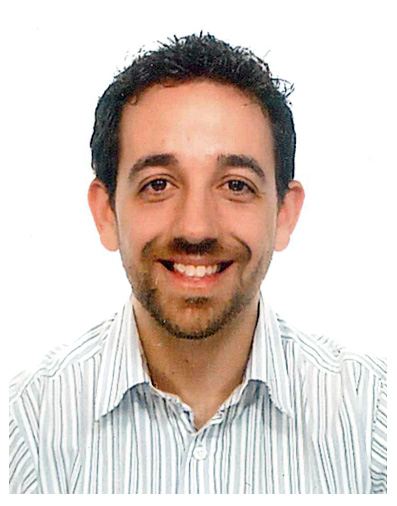
\includegraphics[width=1in,height=1.25in,clip,keepaspectratio]{foto_kike}}]
    {Enrique Mart\'i} is a Senior Researcher on Automated Driving at Tecnalia 
    Research and Innovation since 2017. He received his PhD in Computer Science 
    from University Carlos III de Madrid in 2015. 
    He has more than 10 years of experience in Sensor Fusion and Estimation,
    including participation in R\&D projects and creation of commercial 
    sensor fusion products for UAV/UGV navigation and surveillance systems.
    His research interests include sensor technologies, information fusion,
    machine learning and optimization applied to
    automated vehicles.    
\end{IEEEbiography}

\begin{IEEEbiography}[{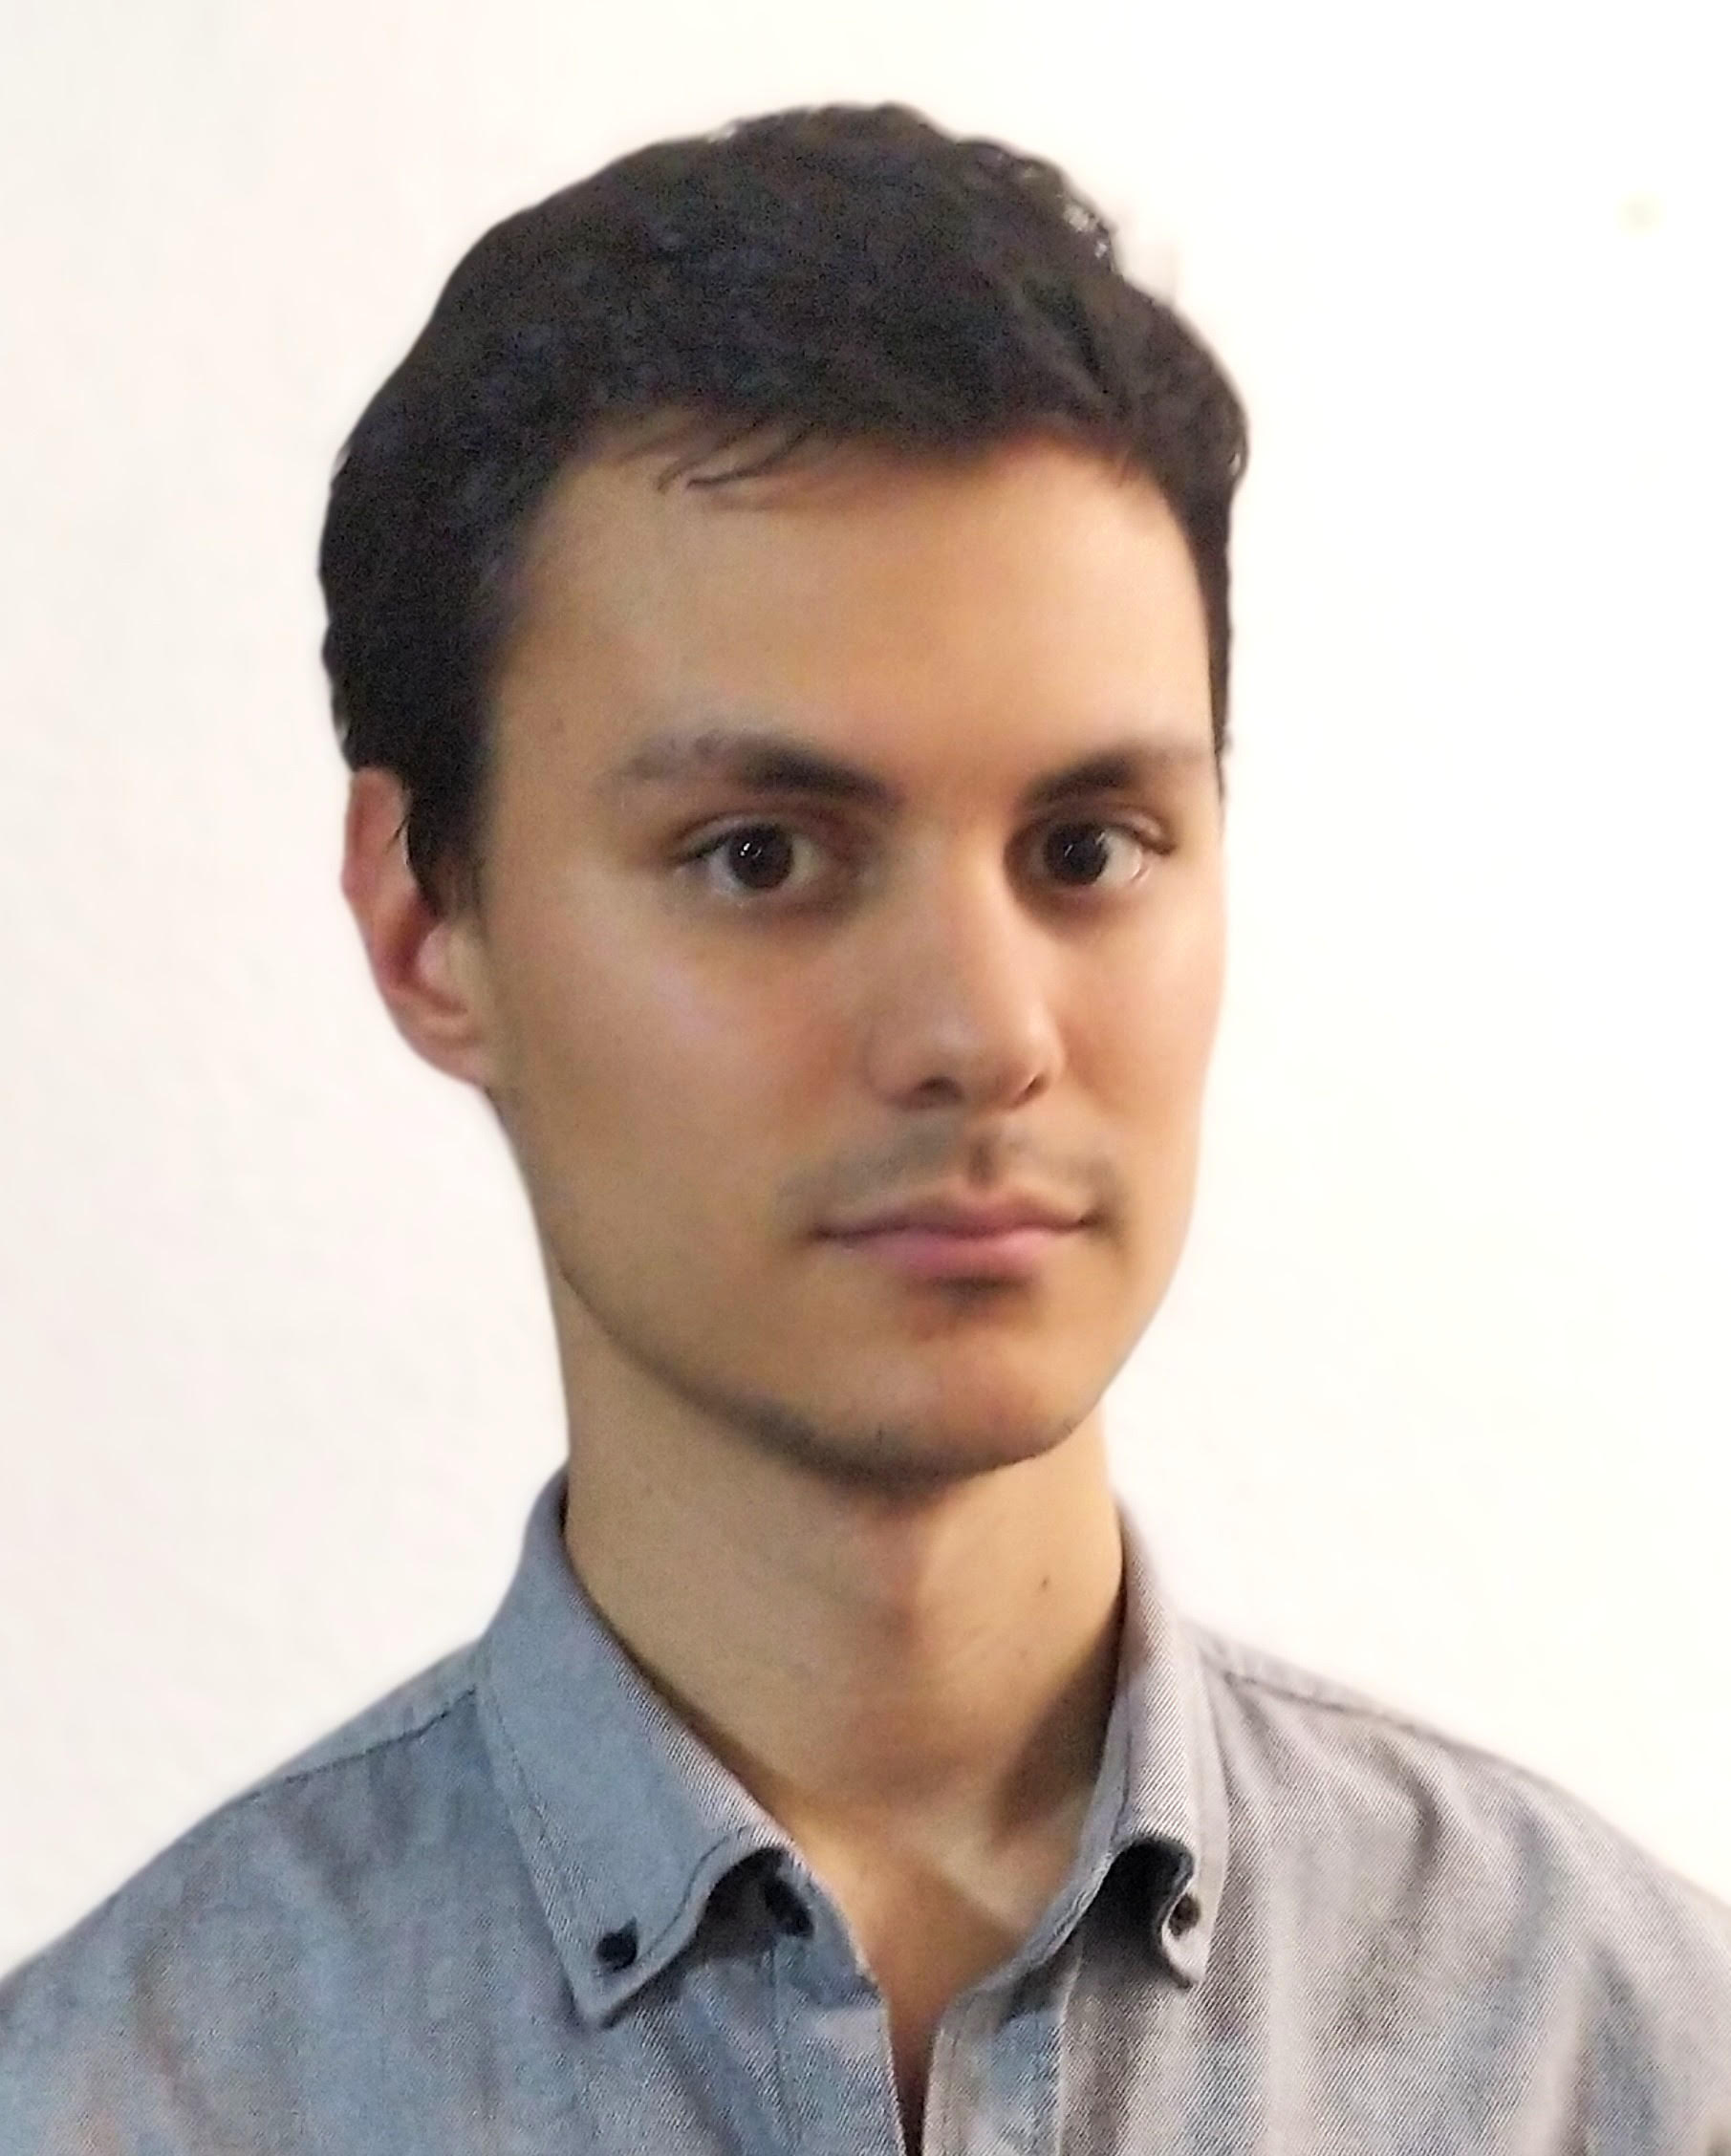
\includegraphics[width=1in,height=1.25in,clip,keepaspectratio]{Foto_miguel}}]
{Miguel \'Angel de Miguel}
is a Ph.D. student and an assistant lecturer at University Carlos III de Madrid.
He received the B.S degree in electronics engineering in 2015 and the M.S. 
degree in industrial
engineering in 2017, both at University Carlos III de Madrid.
In 2013 he joined the Intelligent Systems Lab where he has collaborated
in industrial research projects for four years.
His research interests include the areas of path planning and control 
with a focus on applications for autonomous vehicles.
\end{IEEEbiography}


\begin{IEEEbiography}[{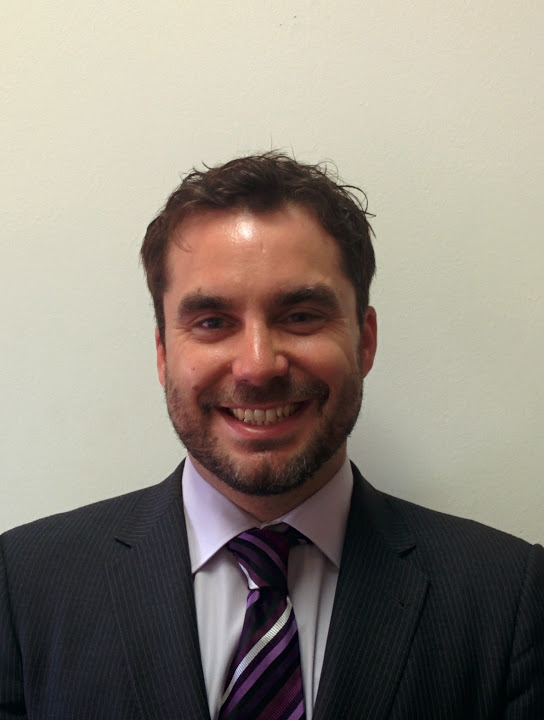
\includegraphics[width=1in,height=1.25in,clip,keepaspectratio]
        {foto_fernando}}]
    {Fernando Garc\'ia} is Professor at Universidad Carlos III de Madrid. His 
    research focus in Intelligent Vehicles and Intelligent 
    Transportation Systems involving the use of Computer Vision, Sensor Fusion, 
    and Human Factors. He 
    %has organization experience in the ITSS conferences and
    is member of the BoG and Vice-president of the Spanish Chapter of the 
    IEEE-ITSS since January 2017. He has been recipient of the Barreiros 
    Foundation Award %in the domain of Automotive and Vehicle Applications 
    in 2014 and finalist to the best PhD Thesis Dissertation Award in the 
    period 2013-2015 given by ITSS Spanish Chapter.   

\end{IEEEbiography}

\begin{IEEEbiography}[{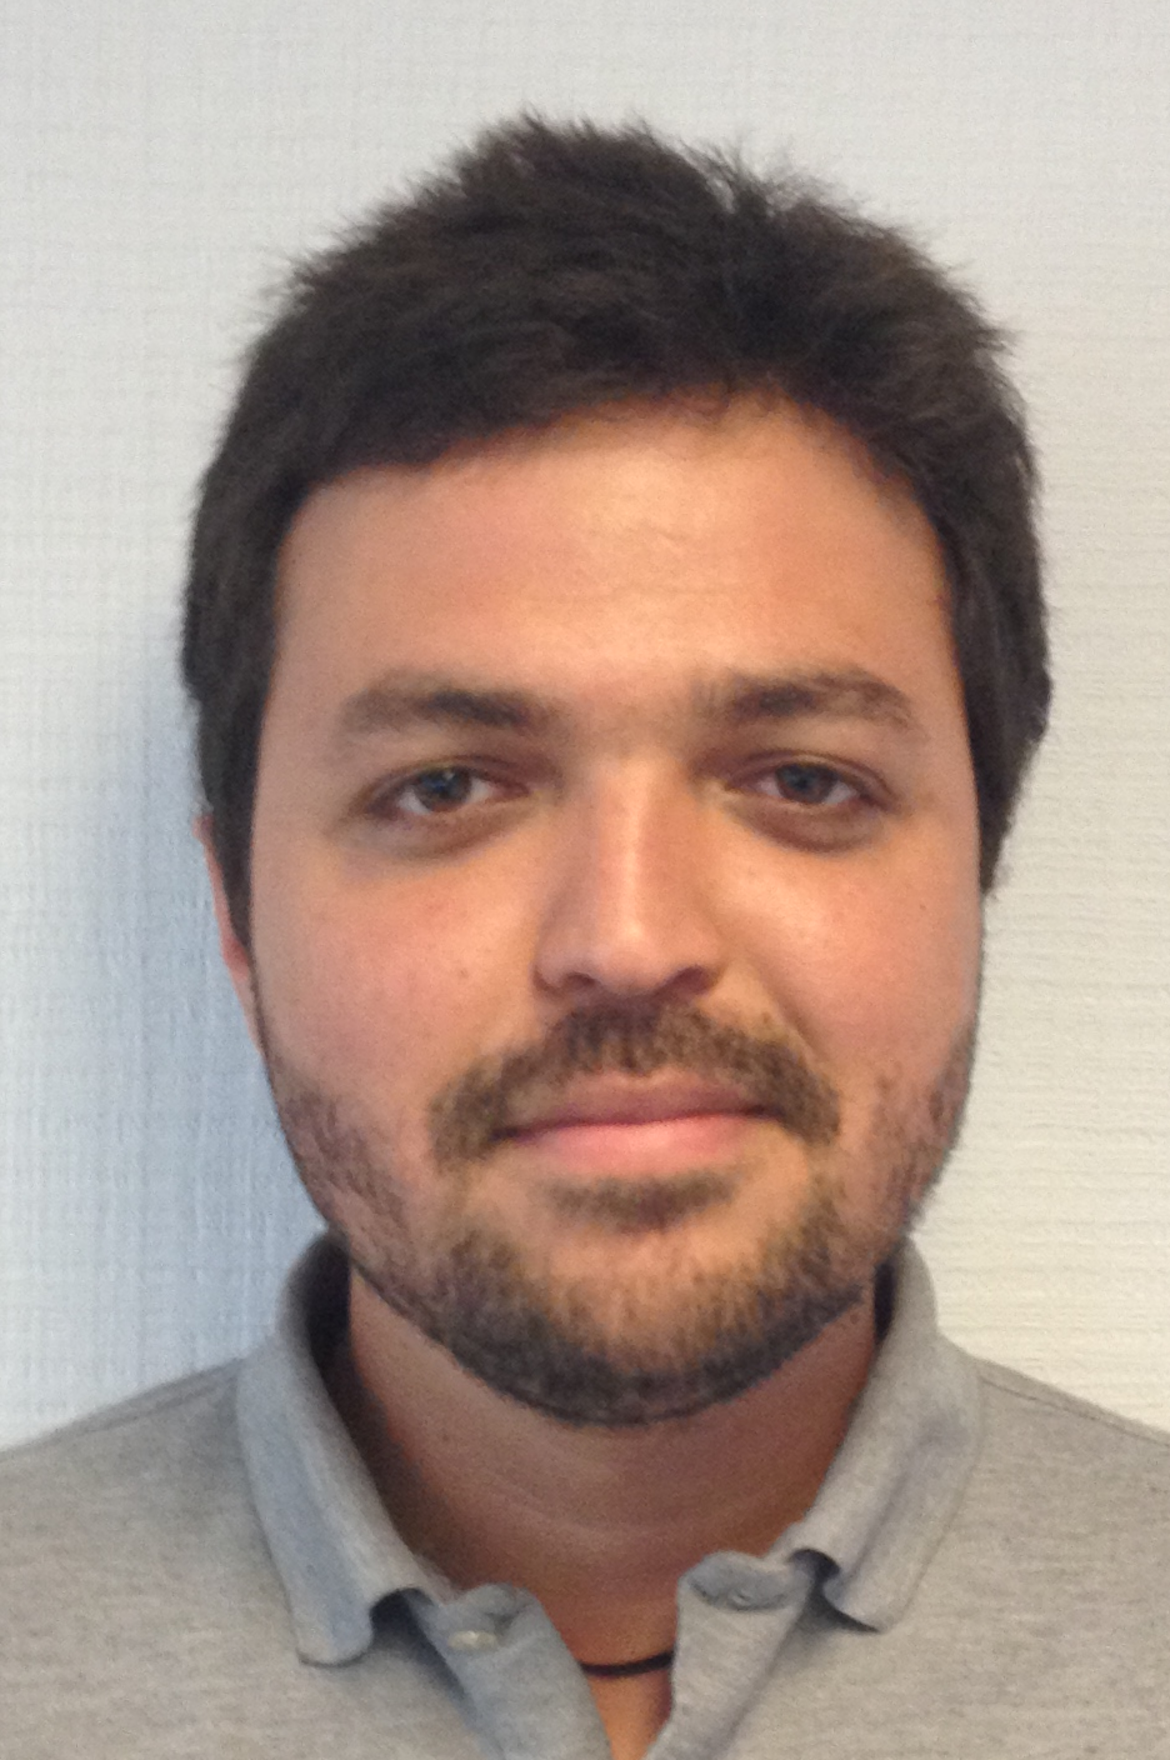
\includegraphics[width=1in,height=1.25in,clip,keepaspectratio]{FotoPaperJosh}}]
    {Joshu\'e P\'erez} is a Research leader on Automated Driving at Tecnalia 
    Research and Innovation, since 2015. He received the B.E. degree in 
    electronic engineering from the Simon Bolívar University, Venezuela, in 
    2007. His M.E. degree and his Ph.D. degree from the University Complutense 
    of Madrid were achieved in 2009 and 2012, respectively. He has more than 11 
    years of experience in the Intelligent Transportation System field, and 
    more than 100 publications related to Automated Driving and ADAS. 
\end{IEEEbiography}


% insert where needed to balance the two columns on the last page with
% biographies
%\newpage

% You can push biographies down or up by placing
% a \vfill before or after them. The appropriate
% use of \vfill depends on what kind of text is
% on the last page and whether or not the columns
% are being equalized.

\vfill

% Can be used to pull up biographies so that the bottom of the last one
% is flush with the other column.
%\enlargethispage{-5in}



% that's all folks
\end{document}


